\documentclass[12pt, git, final]{rureport}


\begin{document} % this tells the compiler that it is time to make
                 % text to print instead of just getting ready.
\maketitle  % make a title page from the Title, Date, and Author

%\fxnote{skoða titil á skýrslu, sbr. forsíðu}

%\section*{Errata} %%section* avoids putting a number 
%
\section{Inngangur} % sections break up the document into pieces
Himingeimurinn er fyrir mörgum jafn áhugaverður og hann er að stærð og menn hafa öldum saman spáð mikið í himintunglum og önnur fyrirbæri út í geimi. Ákveðið var því að ná í gögn fyrir sólmyrkva jarðar, ásamt því að ná í gögn fyrir stríð  sem herjað hefur jörðina og vopnasölu út um heim allan. Fyrst og fremst vildi hópurinn skoða hvernig stríð dreifist á jörðina, hversu oft og hvar lenda sólmyrkvarnari á jörðina meðan stríðin geisa og hvort það sé möguleiki á fylgni milli fjölda sólmyrkva og fjölda stríðsátaka? Þessir útgangspunktar verða skoðaðir nánar og gefin skil á niðurstöðunum. 
\section{Framkvæmd}



\section{Aðferð}
\subsection{Gögn}
Fyrst var farið á veraldarvefin og leitað af gögnum sem hægt væri að vinna með, gögnin voru fundin á síðu á síðu hjá NASA\cite{Eclipse}, Stockholm international peace research institution\cite{weapon} og Háskólanum í Uppsölum í Svíþjóð\cite{conflict}. Gögnin voru tekin inn og unnið með þau í þremur mismunandi skrám.
\subsection{Hönnun}
Við hönnun á GUI þá notast  við Qt4 Designer \cite{qt4}. Ákveðið var að það yrði innskráningar gluggi og þar þarf að skrá inn upplýsingar til að tengjast gagnagrunninum og nota notendaviðmótið.

Við notumst við Basemap\cite{basemap} sem er viðbótarpakki fyrir Matplotlib til að sýna hvernig sólmyrkvinn lendir á jörðinni. Gögnin um sólmyrkvan eru frá NASA og eru þær upplýsingar notaðar til að sýna staðsetningarnar sólmyrkvana á jörðinni, einnig sýnum við að 

\subsection{Virkni}
Virkni forritsins er þannig að notandinn skoðar upplýsingarnar út frá árum og getur annað hvort hreyft stiku til að velja árið sem á að skoða, eða skrifa ártalið beint í glugga, upplýsingarnar skila sér svo í dálka við hliðina.



\section{Niðurstöður}\label{nidurstodur}
Þegar plottaðir voru staðsetningarnar fyrir sólmyrkvana þá sást að lína myndaðist á breiddargráðum 60$^{\circ}$-75$^{\circ}$ bæði á norður- og suðurhveli. og sú lína spannar ca 43,6\% af öllum sólmyrkvunum sem hafa verið á jörðinni frá tímabilinu 1901 - 2100. 


\pagebreak

\begin{figure}
	\centering 
	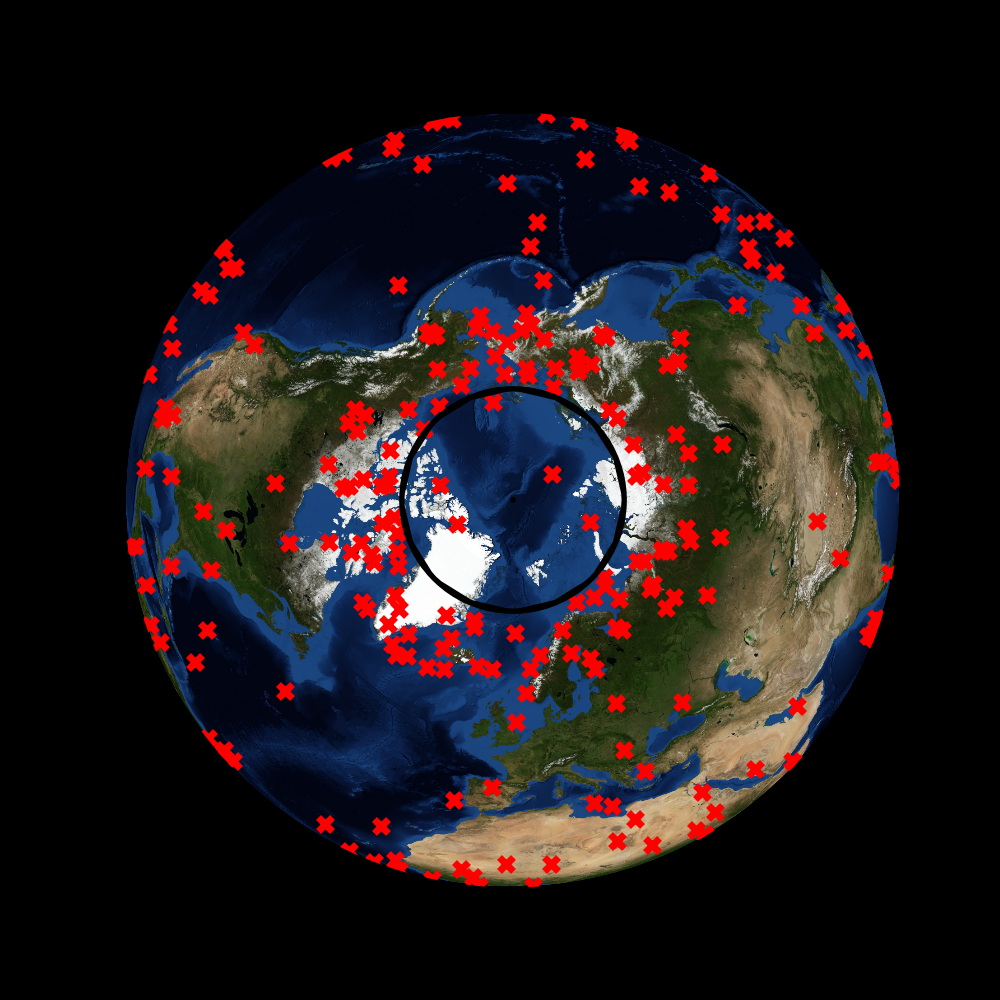
\includegraphics[width=\textwidth]{3D from Northpole.png}
	\caption{Sólmyrkvar séð frá Norður pólnum \label{fig:3DNP}}
\end{figure}

\clearpage

\printbibliography

\end{document} % this tells the compiler that we are done

% These are variables for the editor Emacs
%%% Local Variables: 
%%% TeX-command-BibTeX: biber
%%% mode: latex
%%% TeX-master: t
%%% End:
